\lipsum[1]

\section{Problem Statement / Objectives}
\lipsum[1]

% add images/test.png
\begin{figure}[thb]
    \centering
    \includegraphics[scale=0.1]{images/test.png}
    \caption{Example Image}
    \label{fig:example_image}
\end{figure}

\section{Scope, Methodology, and Design}
%  - Architecture, HLD / LLD, if applicable
\lipsum[1]
\section{Work Done}
% Implementations, Challenges, Mitigations, etc.
\lipsum[1]



\section{Example Section}

\lipsum[1-2]
\lipsum[66]



\subsection{Example Table}

\lipsum[1]

\begin{table}[thb]
    \renewcommand{\arraystretch}{1.3}
    \captionabove{Example Table.}
    \label{table:example_table}
    \centering

    \begin{tabular}{|r|l|}
      \hline
      7C0         & hexadecimal \\
      3700        & octal \\
      \cline{2-2}
      11111000000 & binary \\
      \hline
      \hline
      1984        & decimal \\
      \hline
    \end{tabular}
\end{table}


\lipsum[2-4]



\subsection{Example Plot}

\lipsum[1]

\begin{figure}[thb]
    \centering

    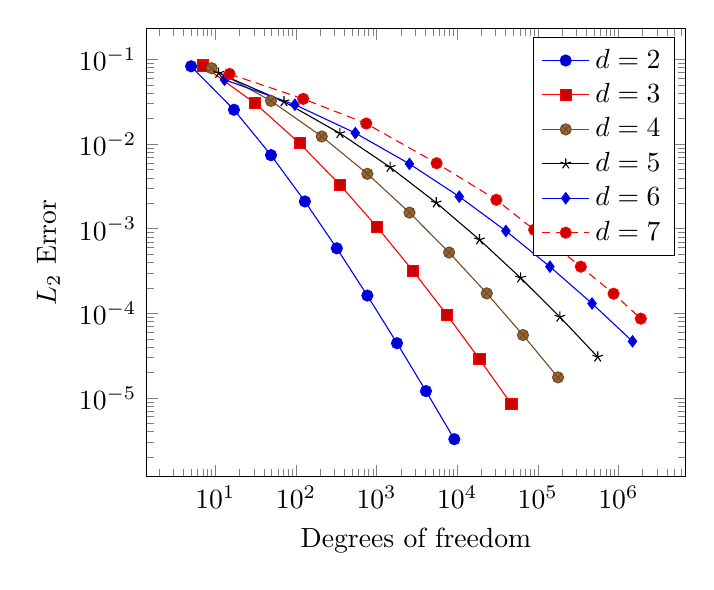
\begin{tikzpicture}
        \begin{loglogaxis}[
            xlabel={Degrees of freedom},
            ylabel={$L_2$ Error}
            ]
            \addplot coordinates {
              (5,8.312e-02)    (17,2.547e-02)   (49,7.407e-03)
              (129,2.102e-03)  (321,5.874e-04)  (769,1.623e-04)
              (1793,4.442e-05) (4097,1.207e-05) (9217,3.261e-06)
            };

            \addplot coordinates{
              (7,8.472e-02)    (31,3.044e-02)    (111,1.022e-02)
              (351,3.303e-03)  (1023,1.039e-03)  (2815,3.196e-04)
              (7423,9.658e-05) (18943,2.873e-05) (47103,8.437e-06)
            };

            \addplot coordinates{
              (9,7.881e-02)     (49,3.243e-02)    (209,1.232e-02)
              (769,4.454e-03)   (2561,1.551e-03)  (7937,5.236e-04)
              (23297,1.723e-04) (65537,5.545e-05) (178177,1.751e-05)
            };

            \addplot coordinates{
              (11,6.887e-02)    (71,3.177e-02)     (351,1.341e-02)
              (1471,5.334e-03)  (5503,2.027e-03)   (18943,7.415e-04)
              (61183,2.628e-04) (187903,9.063e-05) (553983,3.053e-05)
            };

            \addplot coordinates{
              (13,5.755e-02)     (97,2.925e-02)     (545,1.351e-02)
              (2561,5.842e-03)   (10625,2.397e-03)  (40193,9.414e-04)
              (141569,3.564e-04) (471041,1.308e-04) (1496065,4.670e-05)
            };

            \addplot coordinates{
              (15,6.75e-02)     (123,3.425e-02)     (745,1.751e-02)
              (5561,5.942e-03)   (30625,2.197e-03)  (90193,9.714e-04)
              (341569,3.564e-04) (871041,1.708e-04) (1896065,8.670e-05)
            };
            \legend{$d=2$,$d=3$,$d=4$,$d=5$,$d=6$,$d=7$}
        \end{loglogaxis}
    \end{tikzpicture}

    \caption{Example Plot.}

    \label{fig:example_plot}
\end{figure}

\lipsum[3]
\lipsum[66]



\subsection{Example Barchart}

\lipsum[1]

\begin{figure}[thb]
    \centering

    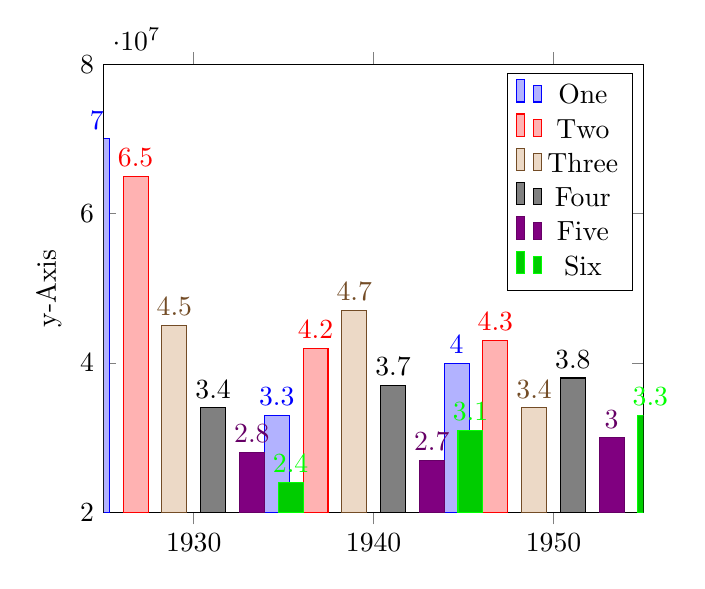
\begin{tikzpicture}
        \begin{axis}[
            ybar               = 5pt, % configures `bar shift'
            xmajorgrids        = false,
            x tick label style = {
              /pgf/number format/1000 sep =},
            xtick              = {1930, 1940, 1950},
            ylabel             = y-Axis,
            enlarge x limits   = 0.25,
            ymin               = 2e7,
            ymax               = 8e7,
            bar width          = 9pt,
            point meta         = y *10^-7, % the displayed number
            nodes near coords,
            ]
            \addplot
            coordinates {(1930,70e6) (1940,33e6)
              (1950,40e6)};

            \addplot
            coordinates {(1930,65e6) (1940,42e6)
              (1950,43e6)};

            \addplot
            coordinates {(1930,45e6) (1940,47e6)
              (1950,34e6)};

            \addplot
            coordinates {(1930,34e6) (1940,37e6)
              (1950,38e6)};

            \addplot
            coordinates {(1930,28e6) (1940,27e6)
              (1950,30e6)};

            \addplot
            coordinates {(1930,24e6) (1940,31e6)
              (1950,33e6)};

            \legend{One, Two, Three, Four, Five, Six}
        \end{axis}
    \end{tikzpicture}

    \caption{Example Barchart.}

    \label{fig:example_barchart}
\end{figure}

\lipsum[3]
\lipsum[66]



\subsection{Example SVG Graphics Input}

\lipsum[1]

\begin{figure}[thb]
  \centering
  \includegraphics{shapes}

  \caption{Example Shapes from an SVG.}
  \label{fig:example_svg}
\end{figure}

\lipsum[42]



\subsection{Example Source Code}

\lipsum[1]

\begin{lstlisting}[
    language = C,
    caption  = {Example Source Code},
    label    = {list:example_src}
]
#include <stdio.h>

void quick_sort (int *a, int n) {
    int i, j, p, t;
    if (n < 2)
        return;
    p = a[n / 2];
    for (i = 0, j = n - 1;; i++, j--) {
        while (a[i] < p)
            i++;
        while (p < a[j])
            j--;
        if (i >= j)
            break;
        t = a[i];
        a[i] = a[j];
        a[j] = t;
    }
    quick_sort(a, i);
    quick_sort(a + i, n - i);
}

/* main routine */
int main (void) {
    int a[] = {4, 65, 2, -31, 0, 99, 2, 83, 782, 1};
    int n = sizeof a / sizeof a[0];
    int i;
    for (i = 0; i < n; i++)
        printf("%d%s", a[i], i == n - 1 ? "\n" : " ");
    quick_sort(a, n);
    for (i = 0; i < n; i++)
        printf("%d%s", a[i], i == n - 1 ? "\n" : " ");
    return 0;
}
\end{lstlisting}



\subsection{Example Subsection}

\lipsum[1]



\subsubsection{Example SubSubSection}

\lipsum[9]



\subsubsection{Example SubSubSection}

\lipsum[10]